
\chapter{CNN}

CNN stands for convolutional neural network.
Convolutional networks are neural networks that have convolutional layers.
A typical convolutional layer consists of three stages:
\begin{enumerate}
\item convolution stage: affine transform
\item detector stage: nonlinearty
\item pooling stage
\end{enumerate}

\section{Convolution}

\begin{equation}
  \label{eq:convolution}
  s(t) = \int x(a)w(t-a)da.
\end{equation}

This operation is called \keyword{convolution}.
The convolution operation is typically denoted with an asterisk:
\begin{equation}
  s(t) = (x*w)(t).
\end{equation}

In convolutional network terminology, the first argument (in this example, the function $x$) to the convolution is often referred to as the \keyword{input}, and the second argument (int this example, the function $w$) as the \keyword{kernel}.
The output is sometimes referred to as the \keyword{feature map}.

If we assume that $x$ and $w$ are defined only on integer $t$, we can define the discrete convolution:
\begin{equation}
  \label{eq:discrete-convolution}
  s(t) = (x*w)(t) = \sum_{a=-\infty}^{\infty} x(a)w(t-a).
\end{equation}

We often use convolutions over more than one axis at a time.
For example, if we use a two-dimensinal image $I$ as our input, we probably also want to use a two-dimensional kernel $K$:
\begin{equation}
  S(i,j) = (I*K)(i,j) = \sum_m\sum_n I(m,n)K(i-m,j-n).
\end{equation}


The following formula can be used to calculate the output dimension.
\begin{gather}
  h_{o} = \frac{h_{i} - h_{k}}{h_{s}} + 1\\
  w_{o} = \frac{w_{i} - w_{k}}{w_{s}} + 1
\end{gather}
where \(h_{o}\) is the output height, \(h_{i}\) is the input height, \(h_{k}\) is the kernel height, \(h_{s}\) is the stride height, \(w_{o}\) is the output width, \(w_{i}\) is the input width, \(w_{k}\) is the kernel width, \(w_{s}\) is the stride width.

The convolution operation is shown in Figure \ref{fig:conv-op}.
\begin{figure}[!htbp]
  \centering
  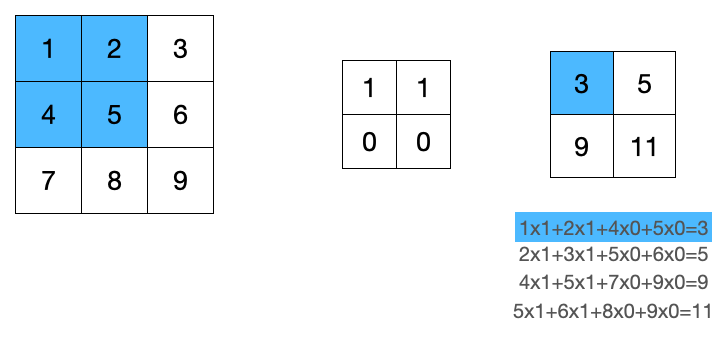
\includegraphics[width=0.8\textwidth]{conv}
  \caption{Convoluation operation}
  \label{fig:conv-op}
\end{figure}
\section{Properties}

CNN leverages three important ideas:
\begin{itemize}
\item sparse interaction.
\item parameter sharing.
\item equivariant representations.
\end{itemize}

\subsection{Sparse interaction}

This is accomplished by making the kernel smaller than the input.


\subsection{Parameter sharing}

In convolutional layers, the same parameter defined in one kernel are used at every position of the input.


\subsection{Equivariant representations}

In the case of convolution, the particular form of a parameter sharing causes the layer to have a property called \keyword{equivariance} to translation.
To say a function is equivariant means that if the input changes, the output changes in the same way.




\section{ Pooling}


A pooling function replaces the output of the net at a certain location with a summary statistic of the nearby outputs.
For example, the max pooling oeration reports the maximum output within a rectangular neighborhood.
Pooling helps to make the representation approximately invariant to small translations of the input.
Invariant to translation means that if we translate the input by a small amount, the values of most of the pooled outputs do not change.

The following formula can be used to calculate the output dimension.
\begin{gather}
  h_{o} = \frac{h_{i} - h_{k}}{h_{s}} + 1\\
  w_{o} = \frac{w_{i} - w_{k}}{w_{s}} + 1
\end{gather}
where \(h_{o}\) is the output height, \(h_{i}\) is the input height, \(h_{k}\) is the pooling height, \(h_{s}\) is the stride height, \(w_{o}\) is the output width, \(w_{i}\) is the input width, \(w_{k}\) is the pooling width, \(w_{s}\) is the stride width.


%%% Local Variables:
%%% mode: latex
%%% TeX-master: "machine-learning"
%%% End:
